\documentclass[border=10pt]{standalone}
\usepackage{tikz}
\usetikzlibrary{arrows.meta, angles, quotes}

\begin{document}
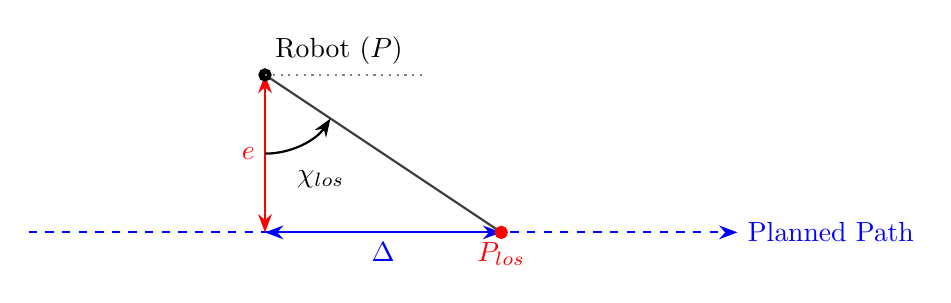
\begin{tikzpicture}[>=Stealth, thick]
    % 定义坐标
    \coordinate (Origin) at (0,0);
    \coordinate (PathEnd) at (8,0);
    \coordinate (P) at (2,2); % 机器人位置
    \coordinate (Projection) at (2,0); % 投影点
    \coordinate (Plos) at (5,0); % LOS 目标点

    % 绘制参考路径
    \draw[->, dashed, blue] (-1,0) -- (PathEnd) node[right] {Planned Path};

    % 绘制横向偏差 e
    \draw[red, <->] (P) -- (Projection) node[midway, left] {$e$};

    % 绘制前视距离 Delta
    \draw[blue, <->] (Projection) -- (Plos) node[midway, below] {$\Delta$};

    % 绘制视线 Line of Sight
    \draw[darkgray, thick] (P) -- (Plos);

    % 绘制机器人和目标点
    \filldraw[black] (P) circle (2pt) node[above right] {Robot ($P$)};
    \filldraw[red] (Plos) circle (2pt) node[below] {$P_{los}$};

    % 绘制角度 chi
    \pic [draw, ->, "$\chi_{los}$", angle eccentricity=1.5, angle radius=1cm] {angle = Projection--P--Plos};

    % 辅助虚线
    \draw[gray, dotted] (P) -- ++(2,0);

\end{tikzpicture}
\end{document}